\chapter{Sprint 3 - Summary}

During sprint 3, four variable pitch mechanisms were assembled with Align T-rex 500 RC helicopter tail mechanisms and the 880KV 3DR motors.(Fig. \ref{fig:before} \& \ref{fig:after} )

\begin{figure}[h]
        \centering
         \begin{minipage}[b]{0.4\textwidth}
            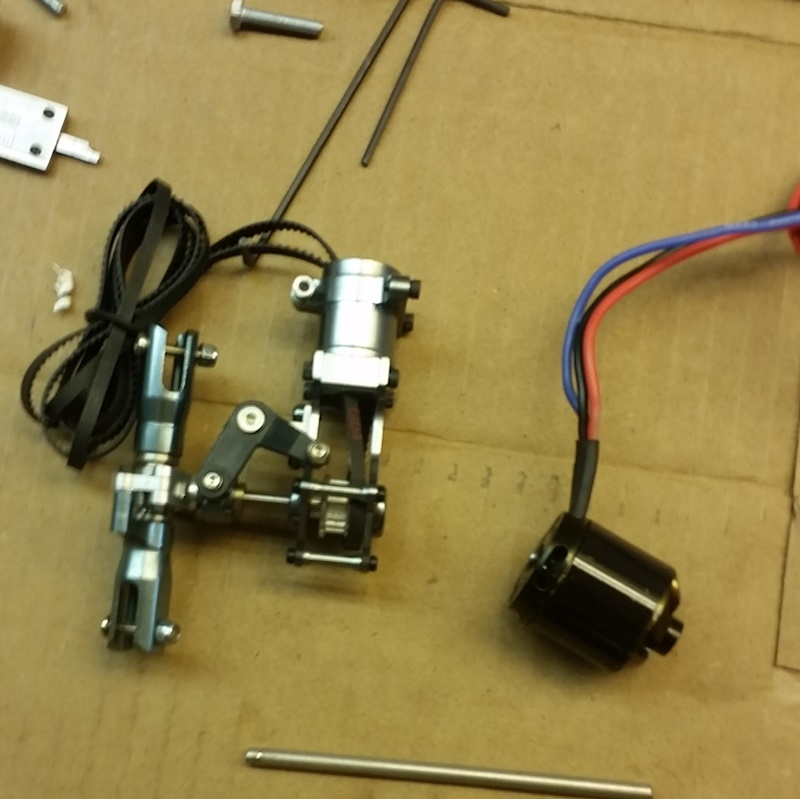
\includegraphics[width = 1\textwidth]{VAPIQ-PICTURES/BeforeAssembly.jpg}
              \caption{Variable Pitch Parts}
            \label{fig:before}
        \end{minipage}
        \hfill
        \begin{minipage}[b]{0.4\textwidth}
            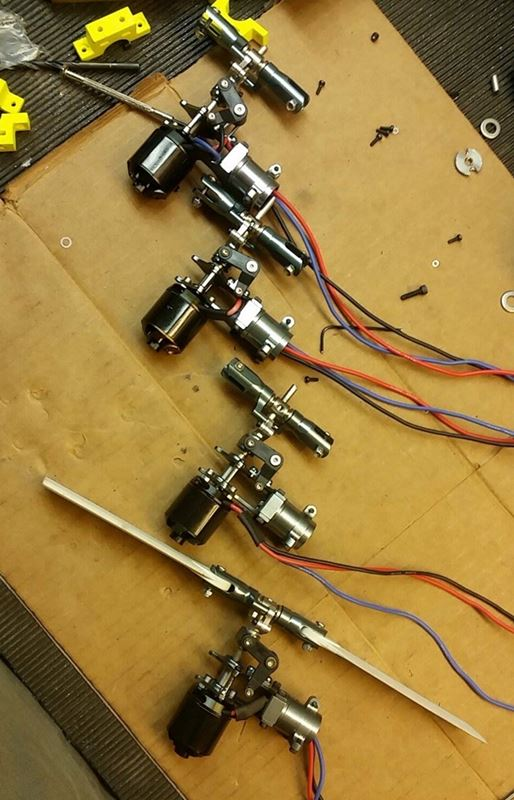
\includegraphics[width = 0.7\textwidth]{VAPIQ-PICTURES/AfterAssemblyVPQ.jpg}
            \caption{Variable Pitch Assembly}
            \label{fig:after}
        \end{minipage}
\end{figure}

The motors from 3DR with 880 KV were mounted straight under the mechanism and a symmetric airfoil capable of generating equal amounts of thrust in each direction were added. The mechanisms function and rotation worked perfectly, but each assembly weighed approximately 175 g each, which adds up to 700g in total. To build a sufficiently functioning quadcopter, thrust to weight ratio should be at least 2:1 as a rule of thumb. Since this was a custom build, it was hard to estimate the lift achievable with this motor-propeller assembly theoretically, therefore a simple thrust test rig was made to measure the actual thrust produced by the motors (Fig. \ref{fig:testrig} \& \ref{fig:testrig2}). 

\begin{figure}[h]
        \centering
         \begin{minipage}[b]{0.4\textwidth}
            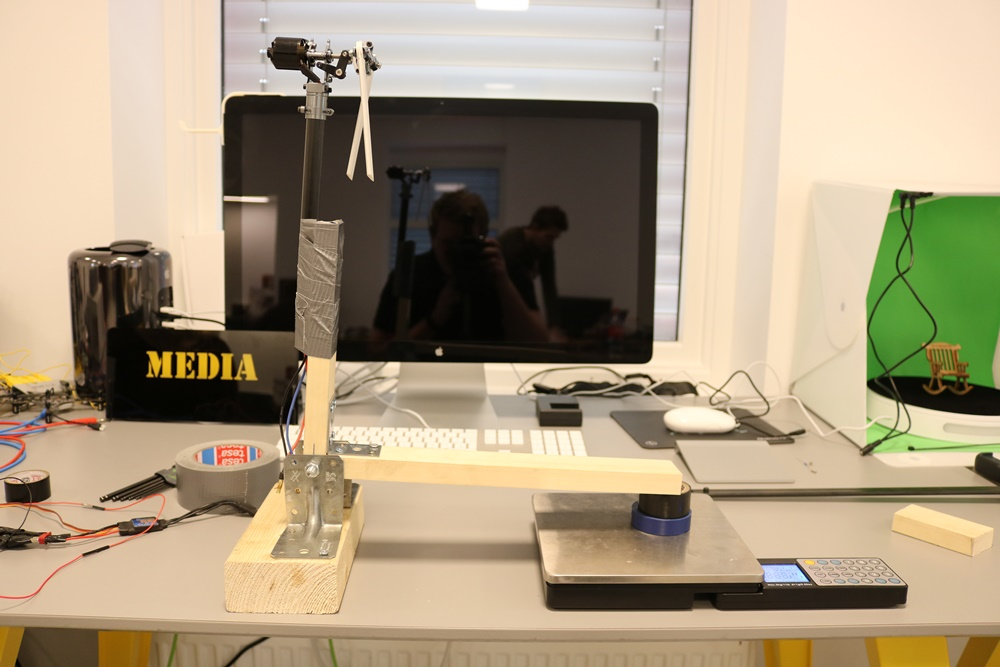
\includegraphics[width = 1\textwidth]{VAPIQ-PICTURES/VPQtestRig}
              \caption{Thrust Test Rig}
            \label{fig:testrig}
        \end{minipage}
        \hfill
        \begin{minipage}[b]{0.4\textwidth}
            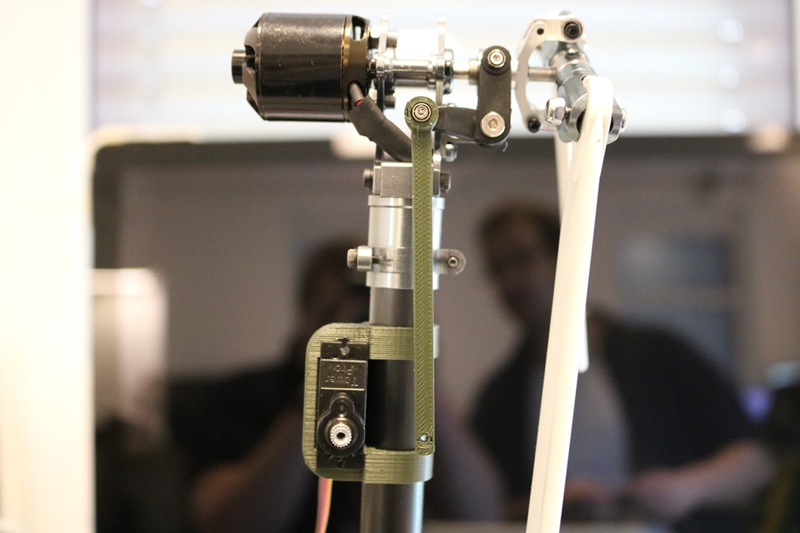
\includegraphics[width = 1\textwidth]{VAPIQ-PICTURES/VpMechanism}
            \caption{Variable Pitch Assembly With Servo}
            \label{fig:testrig2}
        \end{minipage}
\end{figure}

\clearpage 

The measured thrust of the motors was approximately 500 g with 3 cell battery voltage, and 700 g with four cell voltage. This adds up to a maximum thrust of 2,4 kg, while the mass budget for this quadcopter was about 1,8 kg. When using four cell voltage and running at max speed, the motors started to overheat and they consumed a lot of power (18,6Amps on one motor). On this basis, it is not very plausible that this assembly would yield enough lift for the quadcopter. \bigskip

In sprint 3, the team established P-control in the test rig about one axis (Fig. \ref{fig:oneaxis}). The team also established Bluetooth communication with Qualisys. Design wise, there has been generated concepts for the fixed pitch qaudcopter. A new design plan for the variable pitch quadcopter had to be made. The team also investigated several other options for the flight controller. \bigskip

This included planning our own setup as well as looking into the possibility of modifying ArduPilotMega or other existing platforms. The biggest problem of using existing flight controllers is the shear amount of code and interdependencies, and the fact that no open-source controller on the market has functionality that supports variable pitch on quadcopters. \bigskip

The electrical schematics of the components were made for both FPQ and VPQ. The team finally got stable readings from the accelerate and looked into Quaternion based quadcopter modelling. In this sprint, the off board controller was made and started on two axis stabilization. \bigskip

\begin{figure}[h]
        \centering
        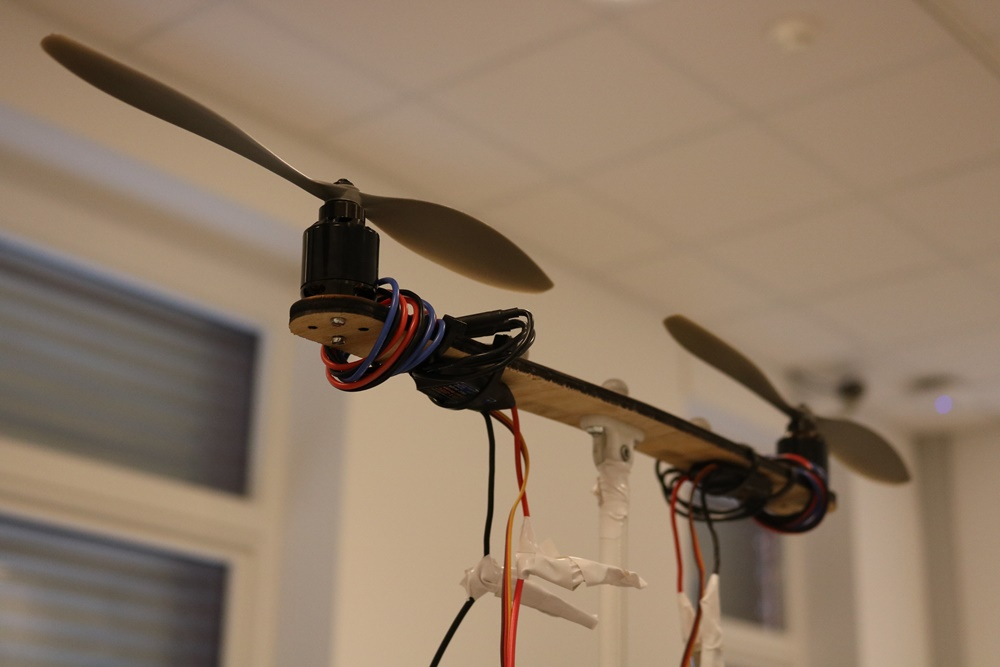
\includegraphics[width = 0.6\textwidth]{VAPIQ-PICTURES/oneaxis}
        \caption{One Axis Test Rig}
        \label{fig:oneaxis}
\end{figure}
  

\newpage
\section{Completion and Scope Change}

In sprint 3, 78\% of the planned tasks were completed and the sprint had a scope change of 16\% (Fig. \ref{fig:bds3}). The change was mainly due to the fact that the assembled mechanisms did not produce enough thrust relative to weight. \\

\textbf{Project plan status, sprint 3:}
\begin{itemize}
    \item Plan Research Paper, \textbf{In progress}
    \item Mechanical Design Plan, Variabel Pitch,  \textbf{Done}
    \item Basic Controller, Fixed Pitch, \textbf{Done}
    \item Motor Control System, Fixed Pitch, \textbf{Done}
    \item Flight Testing And Control, \textbf{In progress}
    \item Mathematical Model, Variable Pitch, \textbf{Done}
    \item Electrical Schematic, Fixed Pitch, \textbf{Done}
    \item Electrical Schematic, Variabe Pitch, \textbf{Done}
\end{itemize}


\begin{figure}[h]
        \centering
        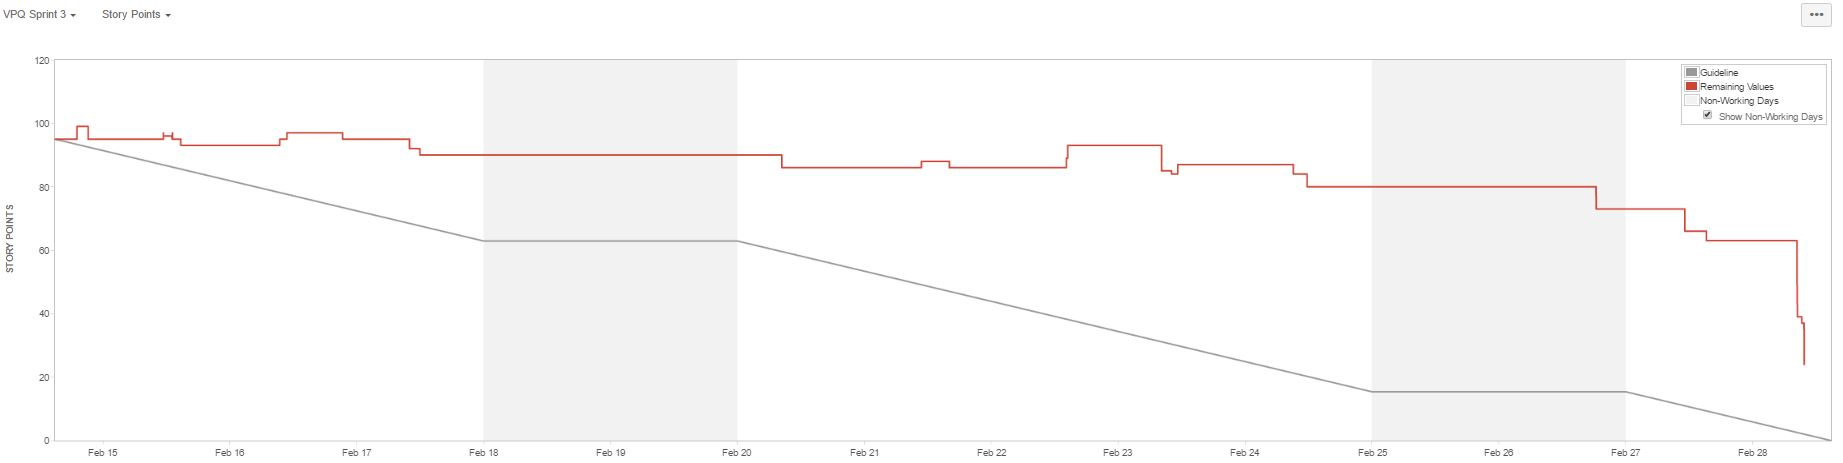
\includegraphics[width = 1\textwidth]{VAPIQ-PICTURES/BDSprint3}
        \caption{Sprint 3 - Burndown Chart}
        \label{fig:bds3}
    \end{figure}
  

%\subsection{Results and Conclusions}


\begin{comment}
The mechanisms made did not work, 
    - off board flight controller
    - Started 2 axis
\section{Challenges}




\section{Lessons Learned}





\end{comment}    






